\documentclass[UTF8]{ctexart}

\title{生物统计课程论文}
\author{Weize Xu}
\date{2019年6月17日}

\usepackage[%
backend=biber,
autocite=superscript,
sorting=none,
style=numeric,
]{biblatex}
\addbibresource{ref.bib}

\usepackage{graphicx}
\usepackage{geometry}
 \geometry{
 a4paper,
 total={170mm,257mm},
 left=20mm,
 top=20mm,
 }

\begin{document}
  \maketitle

  \textbf{摘要}:
  本文探讨了几种机器学习模型在DNA序列分类与回归问题
  上的应用,结合具体的数据集对几种模型的相应问题上的表现进行了
  评估。其中分类问题数据来自于 DAP-Seq 数据得到的
  转录因子结合位点序列数据,回归数据来自于 CRISPR-Cas9 敲除实验
  对癌细胞生长影响数据。通过比较各种方法应用在相应数据上得到的结果,
  讨论了机器学习模型在核酸序列数据的应用方法以及存在的问题。

  \section{前言}
  目前机器学习、统计学习方法已经被广泛应用于DNA序列与基因组学相关实验数据
  的处理、挖掘。机器学习技术大体上可分为需要标签数据的有监督学习技术与
  不需要标签的无监督学习技术。对于有监督学习,两类常见的问题是分类问题和
  回归问题。在基因组数据的机器学习任务上,分类模型常被应用于序列功能预测,
  比如 TF binding site 预测\autocite{ghandi2014enhanced,alipanahi2015predicting}、
  染色质开放区域预测\autocite{kelley2016basset}、
  非编码DNA功能预测\autocite{zhou2015predicting}等问题。
  对于序列数据,由于其本身是非结构化的,无法直接作为特征,
  在训练模型前需要对其进行特征提取, 图\ref{fig:method} (a)。
  根据之前的研究,特征提取根据对信息的利用情况大致上可以分为两类:
  1. 不考虑上下文的特征,比如 k-mer 计数,或者其他在此之上衍生出的
  特征提取技术,比如 gapped k-mer \autocite{ghandi2014enhanced}。
  2. 考虑序列上下文信息的特征提取,比如 sequence embedding \autocite{zeng2018prediction}、
  RNN(递归神经网络)\autocite{shen2018recurrent} 等等。
  一般来说后者由于考虑了更丰富的信息,在数据量充足、问题复杂时
  往往表现出更加优异的结果。但相应的对数据量的要求较高而且计算效率上
  不如前者,所以在实践中还需要结合具体的问题与数据进行选择。

  \section{材料与方法}
  \subsection{数据}
  \subsubsection{分类问题}
  分类问题数据来自于2016年发表于 Nature Biotechnology 的 DAP-Seq 数据\autocite{o2016cistrome}。
  数据包括正样本与负样本共5834条长度为201bp的 DNA 序列。
  其中正样本为实验得出的TF(Transcription Factor,译:转录因子)结合位点附近的DNA序列,负样本为
  染色体上随机抽取的相等长度的序列。

  \subsubsection{回归问题}
  回归问题的数据集来自于CRISPR-Cas9 敲除 p53 enhancer 筛选实验\autocite{korkmaz2016functional}。
  预测的根据为敲除位点附近的核酸序列,预测目标为敲除后癌细胞生长的 Enrichment Z-Score。

  \subsection{序列特征提取}
  \subsubsection{k-mer计数}
  k-mer 计数是一种常用的较为朴素的序列特征提取方法。k-mer 指的是
  序列中长度为 k 的子序列,当序列为DNA时,所有可能的 k-mer 种类
  数量为 $4^k$,所以k-mer 计数特征可表示为一个长度为 $4^k$ 的
  向量 $F_k(s) = [c_1, ... c_i, ... c_{4_k}] $ 其中 $c_i$ 为第 $i$
  个 k-mer 再序列 $s$ 中出现的次数。 对于 k-mer 计数特征,k 是唯一的参数,
  在之前的研究中一般将 k 设置为 6 左右\autocite{ghandi2014enhanced,zeng2018prediction}。

  \subsubsection{k-mer sentence 与 Seq2Vec}
  除了将 k-mer 计数作为序列特征,之前的研究中还有研究者借鉴自然语言
  处理中的方法,将序列视为由 k-mer 作为词的句子。然后将句子嵌入到
  欧式空间中,将嵌入后得到的向量作为特征\autocite{zeng2018prediction}。
  具体的嵌入方法为对sentence中每一个k-mer word的embedding进行优化,
  使得 softmax 函数输入前 n 个words预测接下来出现的word的准确率最大。
  具体细节可参照2018年发表于BMC Genomics上的文献\autocite{zeng2018prediction}。
  最终的实现中采用了Python包 Gensim\autocite{rehurek_lrec} 中的Doc2Vec实现。

  \subsubsection{Recurrent Neural Network}
  既然将DNA序列特征提取能够类比于自然语言序列的特征提取,那么可以进一步
  的借鉴自然语言处理中的其他技术来进行DNA序列特征提取。
  比如使用 RNN (Recurrent Neural Network, 译:递归神经网络)
  或者 LSTM (Long Short-Term Memory)\autocite{hochreiter1997long}、
  GRU(Gated Recurrent Unit)\autocite{cho2014learning}
  等基于神经网络的技术来做特征提取。当然之前已经有研究者使用
  这类技术提取特征用于 TF 结合位点预测\autocite{shen2018recurrent}。

  本文中使用了双向LSTM与注意力机制\autocite{}相结合的神经网络架构,
  见图\ref{fig:method}。它处理
  以 $k=6$ 的 k-mer word 为单位的 k-mer sentence, 提取特征用于序列分类问题。
  双向的LSTM单元用于考虑DNA序列中隐含的上下文信息,注意力单元
  负责为序列中不同的 k-mer 输入分配不同的权重。 网络的参数
  通过 SGD(Stochastic gradient descent, 译:随机梯度下降) 方式进行
  更新。

  \begin{figure}[h!]
  \centering
  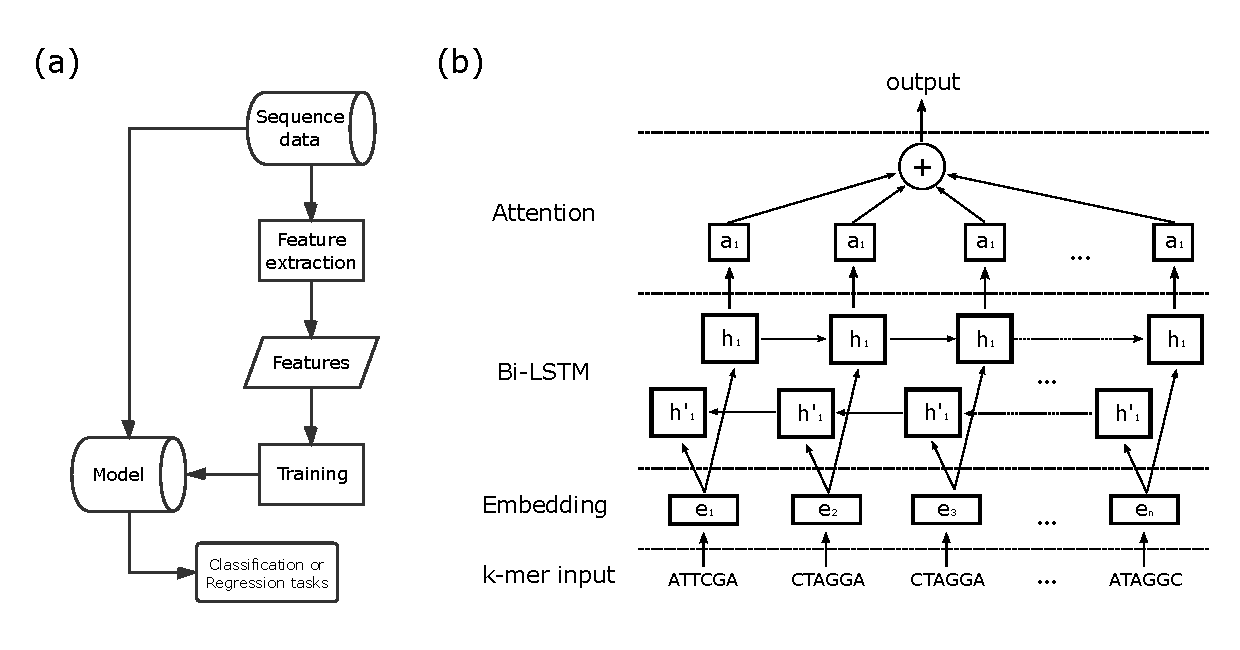
\includegraphics[width=1\textwidth]{imgs/method.pdf}
  \caption{(a) 序列数据相关机器学习任务处理流程图。(b) 本文中使用的双向 LSTM 网络架构示意图。}
  \label{fig:method}
  \end{figure}

  \subsection{分类与回归模型}
  本文中试验的分类器模型有两种:SVM(Support Vector Machine,译:支持向量机)
  与 Random Forest(译:随机森林)。试验的回归模型选择了
  一种线性模型 LASSO(least absolute shrinkage and selection operator)
  与一种基于树的方法 Gradient Boosting Regression Tree。
  超参数选取使用 Grid Search 策略搜索交叉检验中的最优参数。
  由于均为常见统计学习模型,原理此处不再赘述。
  代码实现均来自于 Python 包 Scikit-Learn。

  \subsection{模型选择与结果评价}
  \subsubsection{交叉检验}
  CV(Cross Validation,译:交叉检验)策略被用作模型超参数选择与
  结果评价。在模型选择过程中,首先在样本中划分出test set(测试集),
  然后剩下的部分进行 k-Fold 交叉检验用于模型选择。
  将数据划分为 $k$ 份,然后一次将其中的一份作为 validation set,其他
  作为 training set。进行$k$次训练与测试,选出使得整体结果最优的
  超参数作为最终模型。然后使用 test set 以外的所有数据进行
  模型训练,然后再 test set 上进行测试,对模型进行评价。 

  \subsubsection{分类结果评价}
  在二分类试验中,分类结果可划分为四类:TP(True Positive,真阳性)、
  FP(False Positive,假阳性)、TN(True Negative,真阴性)、
  FN(False Negative,假阴性)。 由此,可以计算以下指标作为分类结果
  好坏的评价:1. ACC(准确率)用于衡量总体分类正确样本所占比例,
  $ACC = \frac{TP + TF}{TP+FP+TN+FN}$。
  2. Precision(精确度)衡量被分类为阳性的结果中TP所占比例,
  $precision = \frac{TP}{TP+FP}$。
  3. Recall(召回率)衡量被分类为阴性的结果中TN所占比例,
  $recall = \frac{TN}{TN+FN}$。
  4. $F_1$ 为 Precision 与 Recall 的调和平均数,对二者权衡考虑,
  $F_1 = (\frac{recall^{-1}+precision^{-1}}{2})^{-1} = \frac{2TP}{2TP+FP+FN}$。
  5. ROC AUC (Receiver Operating Characteristic Area Under Curve) 
  ROC曲线为通过改变判断阈值,使得假阳性率与真阳性率不断发生变化而得到的曲线。
  该曲线下的面积可作为二分类结果好坏的一个不受判定阈值影响的衡量标准。

  \subsubsection{回归结果评价}
  对于回归试验的结果,主要考察的指标有两个。
  1. MSE(Mean Square Error)为真实结果与模型预测结果之差的平方均值,
  $MSE = \frac{1}{n} \sum_{i=1}^{n}{(Y_i - \hat{Y}_i)^2}$。
  数值越小代表回归模型对数据的拟合越小。
  2. $R^2$ 用来衡量模型所解释的变异占数据总变异的比例,越接近于 1 代表
  回归模型对数据变异的解释越好。定义为:
  $R^2 = 1 - \frac{SS_{res}}{SS_{tot}}$,其中
  $SS_{tot} = \sum_{i}{y_i - \overline{y}}$ 为总体变异量,
  $SS_{res} = \sum_{i}{y_i - \hat{y_i}}$ 为模型解释后剩下的变异量。

  \section{结果}
  \subsection{分类问题}
  分类问题的评价结果见表1,
  从中可以看出,基于 k-mer 计数特征训练出的分类器可以很好的解决该问题,
  AUC 可以达到接近 99\% ,而 Seq2Vec 提取到的特征训练出的分类器
  分类的结果反而不如 k-mer 计数,这可能是由于样本数量不能满足需要导致的。
  而双向 LSTM 在这个问题上也可以得到很好的结果。在测试数据集上的 ROC 曲线
  见图\ref{fig:result}(a)-(c)。

  \begin{table}[h]
    \label{tab:res_clf}
    \begin{tabular}{llllll}
    \hline
    Model                   & ACC           & Precision     & Recall        & F1            & AUC           \\ \hline
    k-mer + SVM             & 0.9657$\pm$0.0043 & 0.9654$\pm$0.0077 & 0.9646$\pm$0.0059 & 0.9650$\pm$0.0043 & 0.9906$\pm$0.0031 \\
    k-mer + Random Forest   & 0.9650$\pm$0.0086 & 0.9621$\pm$0.0080 & 0.9668$\pm$0.0134 & 0.9644$\pm$0.0088 & 0.9909$\pm$0.0037 \\
    Seq2Vec + SVM           & 0.8120$\pm$0.0177 & 0.8077$\pm$0.0212 & 0.8094$\pm$0.0211 & 0.8084$\pm$0.0177 & 0.8958$\pm$0.0112 \\
    Seq2Vec + Random Forest & 0.7520$\pm$0.0151 & 0.7632$\pm$0.0115 & 0.7160$\pm$0.0313 & 0.7386$\pm$0.0194 & 0.8330$\pm$0.0130 \\
    Bi-LSTM + Softmax       & 0.9358$\pm$0.0915 & 0.9317$\pm$0.1067 & 0.9519$\pm$0.0480 & 0.9402$\pm$0.0795 & 0.9602$\pm$0.0624 \\ \hline
    \end{tabular}
    \caption{分类问题各模型10Fold交叉检验各检验指标的均值与标准差。}
  \end{table}

  \begin{figure}[h!]
  \centering
  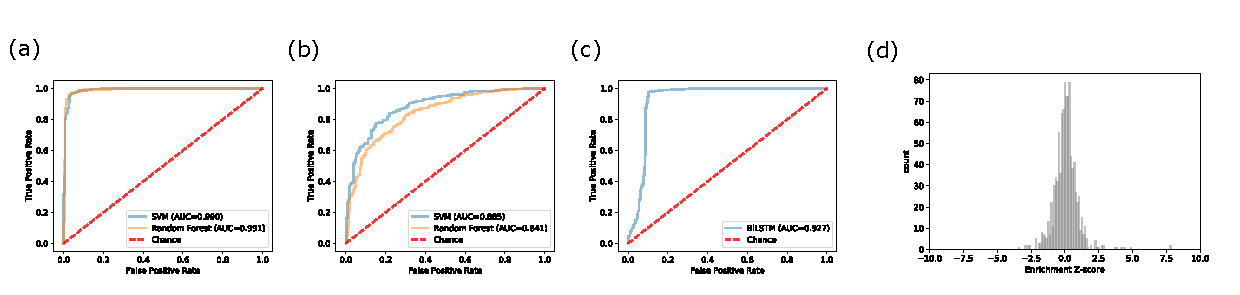
\includegraphics[width=1\textwidth]{imgs/result.pdf}
  \caption{(a)-(c) 分类问题在测试数据集上的 ROC 曲线,从左至右对应 k-mer 计数、Seq2Vec、LSTM。
  (d) 回归问题中 Enrichment-Zscore 的分布。}
  \label{fig:result}
  \end{figure}

  \subsection{回归问题}
  回归问题的评价结果见表2,
  从目前的结果来看,$R^2$ 小于0且波动较大,模型无法对数据趋势进行拟合。
  即使尝试不同的特征序列长度,该回归问题还是无法得到很好的求解。
  分析原因可能是数据中含有的信息量不足,从对该数据集的
  统计中(图\ref{fig:result}(d))可以看出,大多数样本的 Enrichment score 较低,
  分布在$[-2.5, 2.5]$之内,仅有少量(约1.8\%)的样本在此范围外。
  此外,样本的数量很少只有 1000 左右。而 k-mer 特征具有较高的维度,
  导致样本在空间中过于稀疏。

  \begin{table}[h]
  \begin{tabular}{llll}
  \hline
  Model            & seq length: 51                                                           & seq length: 101                                                          & seq length: 201                                                          \\ \hline
  k-mer + Lasso    & \begin{tabular}[c]{@{}l@{}}0.9278$\pm$1.4552\\ -30.4784$\pm$23.1083\end{tabular} & \begin{tabular}[c]{@{}l@{}}0.9278$\pm$1.4552\\ -30.4784$\pm$23.1083\end{tabular} & \begin{tabular}[c]{@{}l@{}}0.9278$\pm$1.4552\\ -30.4784$\pm$23.1083\end{tabular} \\
  k-mer + GBTree   & \begin{tabular}[c]{@{}l@{}}0.9986$\pm$1.3768\\ -58.5660$\pm$38.4751\end{tabular} & \begin{tabular}[c]{@{}l@{}}1.0926$\pm$1.4189\\ -73.7684$\pm$60.0907\end{tabular} & \begin{tabular}[c]{@{}l@{}}1.0668$\pm$1.3994\\ -71.9895$\pm$48.3185\end{tabular} \\
  Seq2Vec + Lasso  & \begin{tabular}[c]{@{}l@{}}0.9278$\pm$1.4552\\ -30.4784$\pm$23.1083\end{tabular} & \begin{tabular}[c]{@{}l@{}}0.9278$\pm$1.4552\\ -30.4784$\pm$23.1083\end{tabular} & \begin{tabular}[c]{@{}l@{}}0.9278$\pm$1.4552\\ -30.4784$\pm$23.1083\end{tabular} \\
  Seq2Vec + GBTree & \begin{tabular}[c]{@{}l@{}}0.9921$\pm$1.3925\\ -55.4674$\pm$27.9595\end{tabular} & \begin{tabular}[c]{@{}l@{}}1.0401$\pm$1.4636\\ -59.5471$\pm$42.9350\end{tabular} & \begin{tabular}[c]{@{}l@{}}1.0500$\pm$1.4468\\ -63.9507$\pm$30.7841\end{tabular} \\
  BiLSTM           & \begin{tabular}[c]{@{}l@{}}1.0753$\pm$0.5401\\   -0.0713$\pm$0.0512\end{tabular} & \begin{tabular}[c]{@{}l@{}}1.0792$\pm$0.2081\\   -0.0638$\pm$0.0333\end{tabular} & \begin{tabular}[c]{@{}l@{}}1.0808$\pm$0.3321\\  -0.0610$\pm$0.0219\end{tabular} \\ \hline
  \end{tabular}
  \label{tab:res_reg}
  \caption{表格中列举了三种不同长度特征序列在几种不同模型上的回归效果。
  格中第一行为MSE的均值与标准差,第二行为$R^2$的均值与标准差。}
  \end{table}

  \section{讨论}
  本文在两个序列相关的统计学习问题数据集上进行了研究。
  讨论了三种对DNA序列数据进行特征提取的方法:k-mer 计数、
  Sequence embedding 与 递归神经网络。 并对在相应的数据
  上进行了实际测试。

  其中分类数据
  使用k-mer 计数方法进行特征提取后给分类器进行学习能够取得很好的效果。
  而后两种特征提取方法的结果反而不如 k-mer 计数, 
  可能的原因是数据量不够。
  而对于回归问题,本文中试验的方法无法很好的对其进行拟合。
  可能的原因有: 1. 数据量不够,由于序列的可变性较高,对于
  长度为 n 的序列,多样性有 $4^n$ 种,且 k-mer 特征的维度较高
  而样本数目过少很可能使得数据过于稀疏,难以对其进行拟合。
  2. 数据中的信息量不足,通过对样本数据的统计,可以看到
  大多数样本的 y 值(Enrichment Z-score)在很小的范围内波动,
  仅有少量样本具有较大的 y 值。
  3. 序列敲除后的效应无法简单通过序列信息进行预测,也许仅仅是DNA序列
  信息不足以推测敲除后带来的表型。需要结合其他种类数据,比如 ChIP-Seq 试验数据等等。

  针对以上分析,几种可能的改进:1. 收集更多的可靠的实验数据。
  2. 进行数据增强,在训练集中将具有较高 y 值的数据对应的序列
  做单碱基的改变,增加其在训练集中所占的比例,提升信息量。
  3. 以公开数据库中的数据为基础(如ENCODE数据库),
  综合敲除位点附近该细胞系的 ChIP-Seq 数据(如组蛋白修饰、转录因子结合等等),将其作为输入,
  增加信息量。
  4. 在增加数据量的同时,试验其他特征提取方法与回归模型。
 
  \printbibliography

\end{document}